\documentclass{standalone}
\usepackage{tikz}
\usetikzlibrary{patterns, positioning}
\usepackage[sfdefault]{ClearSans} %% option 'sfdefault' activates Clear Sans as the default text font
\usepackage[T1]{fontenc}

\begin{document}
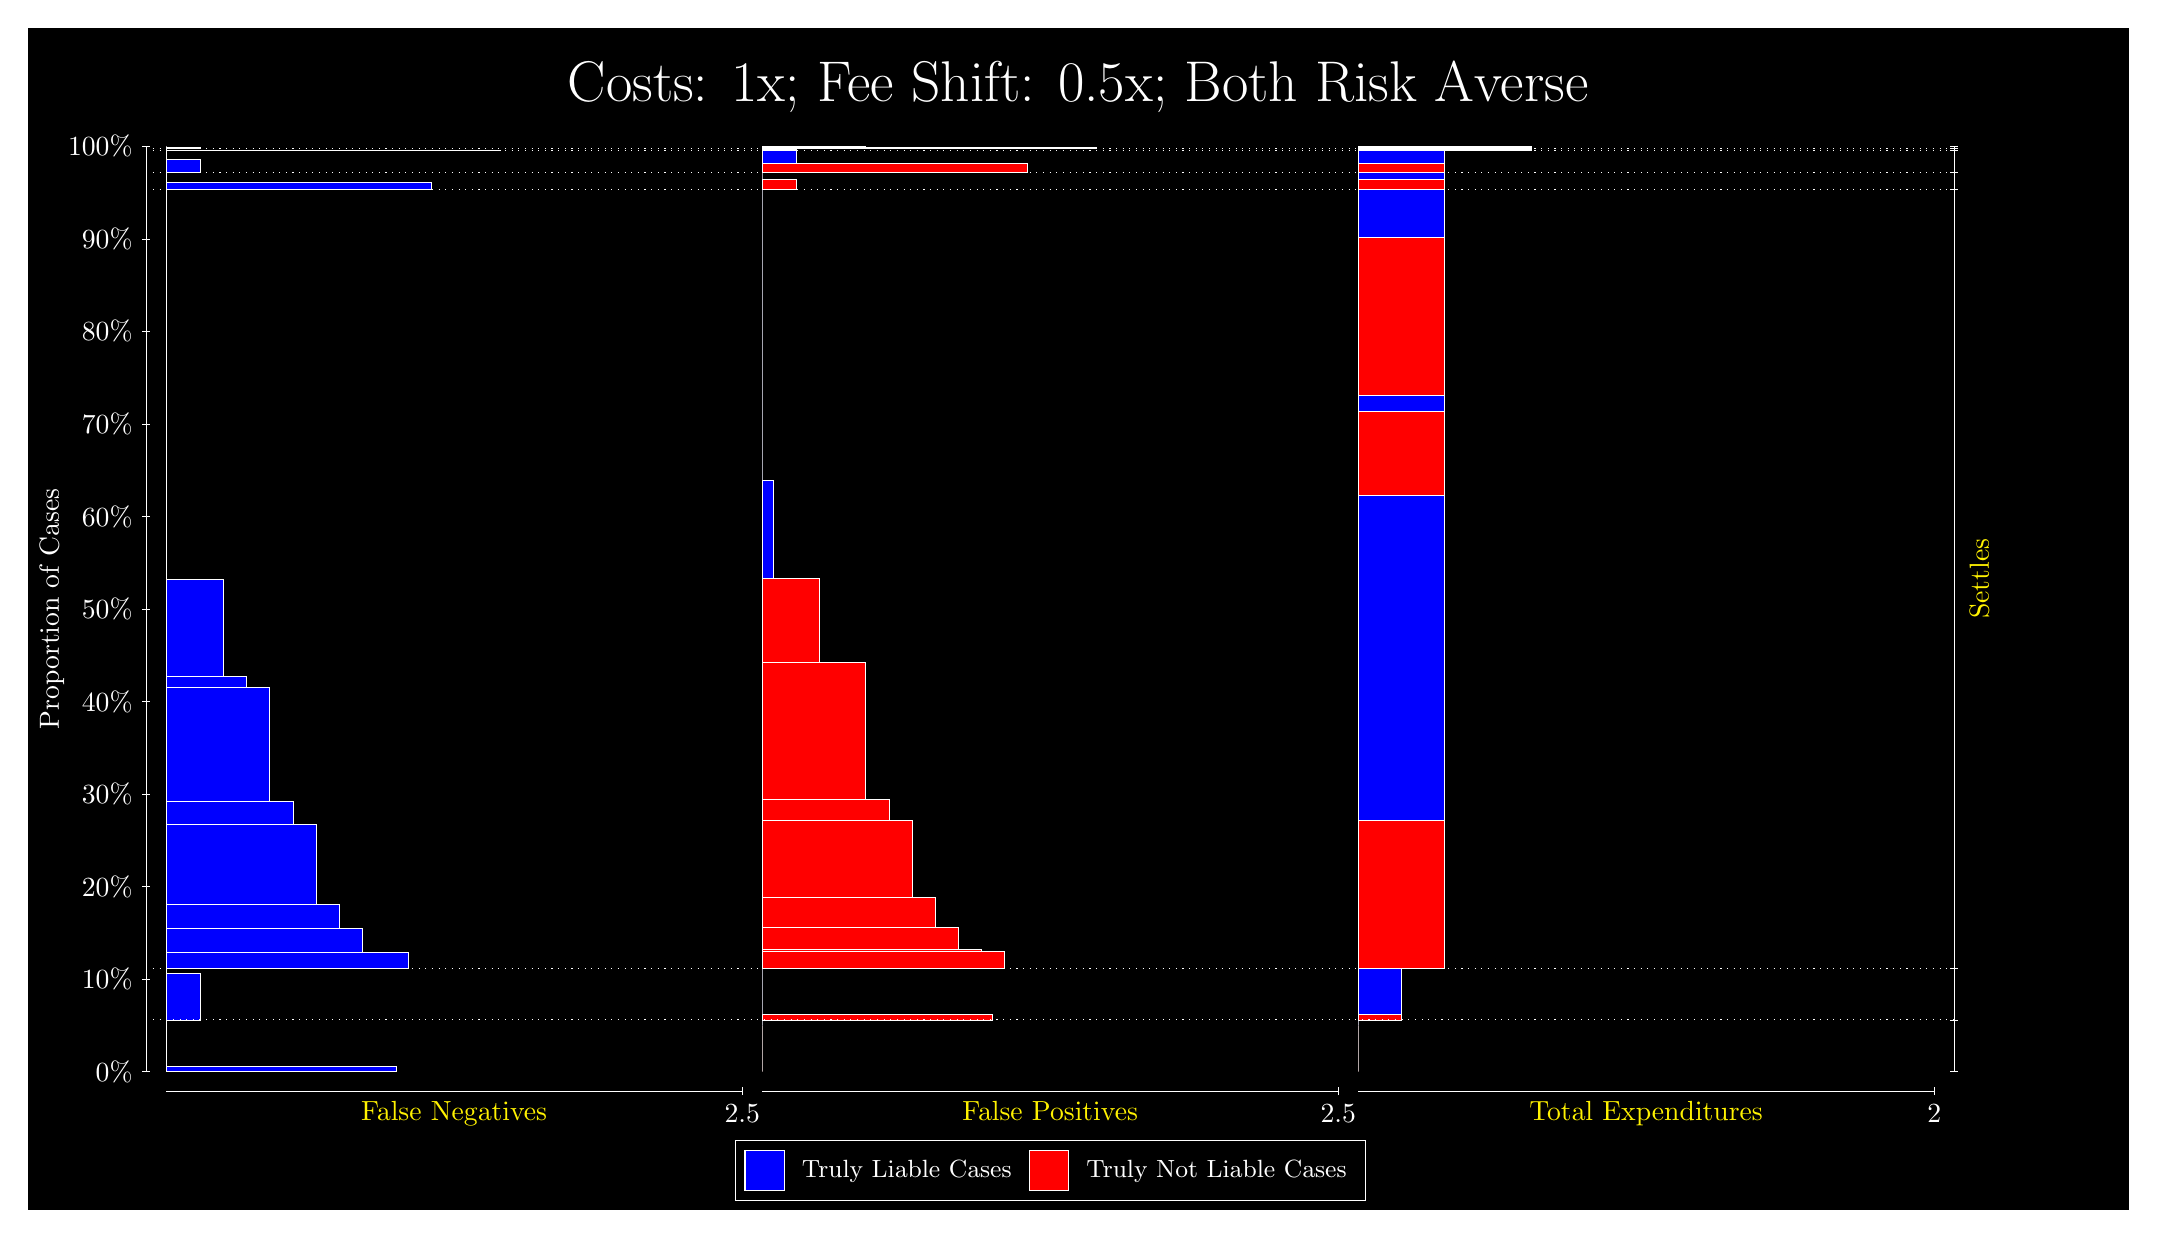
\begin{tikzpicture}
\draw[fill=black] (0,0) rectangle (26.667,15);
\draw[text=white] (0,13.5) rectangle (26.667,15) node[midway] {\huge Costs: 1x; Fee Shift: 0.5x; Both Risk Averse};
\draw[white, very thin] (1.5,1.75) -- (1.5,13.5);
\node[rotate=90, text=white, anchor=center] at (0.3, 7.625) {Proportion of Cases};
\draw[white, very thin] (1.45,1.75) -- (1.55,1.75);
\node[text=white, anchor=east] at (1.45, 1.75) {0\%};
\draw[white, very thin] (1.45,2.925) -- (1.55,2.925);
\node[text=white, anchor=east] at (1.45, 2.925) {10\%};
\draw[white, very thin] (1.45,4.1) -- (1.55,4.1);
\node[text=white, anchor=east] at (1.45, 4.1) {20\%};
\draw[white, very thin] (1.45,5.275) -- (1.55,5.275);
\node[text=white, anchor=east] at (1.45, 5.275) {30\%};
\draw[white, very thin] (1.45,6.45) -- (1.55,6.45);
\node[text=white, anchor=east] at (1.45, 6.45) {40\%};
\draw[white, very thin] (1.45,7.625) -- (1.55,7.625);
\node[text=white, anchor=east] at (1.45, 7.625) {50\%};
\draw[white, very thin] (1.45,8.8) -- (1.55,8.8);
\node[text=white, anchor=east] at (1.45, 8.8) {60\%};
\draw[white, very thin] (1.45,9.975) -- (1.55,9.975);
\node[text=white, anchor=east] at (1.45, 9.975) {70\%};
\draw[white, very thin] (1.45,11.15) -- (1.55,11.15);
\node[text=white, anchor=east] at (1.45, 11.15) {80\%};
\draw[white, very thin] (1.45,12.325) -- (1.55,12.325);
\node[text=white, anchor=east] at (1.45, 12.325) {90\%};
\draw[white, very thin] (1.45,13.5) -- (1.55,13.5);
\node[text=white, anchor=east] at (1.45, 13.5) {100\%};

\draw[white, very thin] (24.457,1.75) -- (24.457,13.5);
\draw[white, very thin] (24.407,1.75) -- (24.507,1.75);
\node[anchor=west] at (24.407, 1.75) {};
\draw[white, very thin] (24.407,2.4059) -- (24.507,2.4059);
\node[anchor=west] at (24.407, 2.4059) {};
\draw[white, very thin] (24.407,3.0617) -- (24.507,3.0617);
\node[anchor=west] at (24.407, 3.0617) {};
\draw[white, very thin] (24.407,12.957) -- (24.507,12.957);
\node[anchor=west] at (24.407, 12.957) {};
\draw[white, very thin] (24.407,13.173) -- (24.507,13.173);
\node[anchor=west] at (24.407, 13.173) {};
\draw[white, very thin] (24.407,13.448) -- (24.507,13.448);
\node[anchor=west] at (24.407, 13.448) {};
\draw[white, very thin] (24.407,13.474) -- (24.507,13.474);
\node[anchor=west] at (24.407, 13.474) {};
\draw[white, very thin] (24.407,13.5) -- (24.507,13.5);
\node[anchor=west] at (24.407, 13.5) {};

\draw[white, very thin, fill=blue] (1.75,1.75) rectangle (4.6775,1.819);
\draw[white, very thin, fill=red] (1.75,1.819) rectangle (1.75,2.4059);
\draw[white, very thin, fill=blue] (1.75,2.4059) rectangle (2.1891,2.9927);
\draw[white, very thin, fill=red] (1.75,2.9927) rectangle (1.75,3.0617);
\draw[white, very thin, fill=blue] (1.75,3.0617) rectangle (4.8239,3.2583);
\draw[white, very thin, fill=blue] (1.75,3.2583) rectangle (4.2384,3.5714);
\draw[white, very thin, fill=blue] (1.75,3.5714) rectangle (3.9457,3.8743);
\draw[white, very thin, fill=blue] (1.75,3.8743) rectangle (3.6529,4.8877);
\draw[white, very thin, fill=blue] (1.75,4.8877) rectangle (3.3602,5.1881);
\draw[white, very thin, fill=blue] (1.75,5.1881) rectangle (3.0674,6.6268);
\draw[white, very thin, fill=blue] (1.75,6.6268) rectangle (2.7746,6.7659);
\draw[white, very thin, fill=blue] (1.75,6.7659) rectangle (2.4819,8.0011);
\draw[white, very thin, fill=red] (1.75,8.0011) rectangle (1.75,12.957);
\draw[white, very thin, fill=blue] (1.75,12.957) rectangle (5.1167,13.049);
\draw[white, very thin, fill=red] (1.75,13.049) rectangle (1.75,13.173);
\draw[white, very thin, fill=blue] (1.75,13.173) rectangle (2.1891,13.336);
\draw[white, very thin, fill=red] (1.75,13.336) rectangle (1.75,13.448);
\draw[white, very thin, fill=blue] (1.75,13.448) rectangle (5.9949,13.456);
\draw[white, very thin, fill=red] (1.75,13.456) rectangle (1.75,13.474);
\draw[white, very thin, fill=blue] (1.75,13.474) rectangle (2.1891,13.492);
\draw[white, very thin, fill=red] (1.75,13.492) rectangle (1.75,13.5);
\draw[white, very thin, fill=red] (9.3189,1.75) rectangle (9.3189,2.3369);
\draw[white, very thin, fill=blue] (9.3189,2.3369) rectangle (9.3189,2.4059);
\draw[white, very thin, fill=red] (9.3189,2.4059) rectangle (12.246,2.4749);
\draw[white, very thin, fill=blue] (9.3189,2.4749) rectangle (9.3189,3.0617);
\draw[white, very thin, fill=red] (9.3189,3.0617) rectangle (12.393,3.2772);
\draw[white, very thin, fill=red] (9.3189,3.2772) rectangle (12.1,3.2993);
\draw[white, very thin, fill=red] (9.3189,3.2993) rectangle (11.807,3.5788);
\draw[white, very thin, fill=red] (9.3189,3.5788) rectangle (11.515,3.96);
\draw[white, very thin, fill=red] (9.3189,3.96) rectangle (11.222,4.9423);
\draw[white, very thin, fill=red] (9.3189,4.9423) rectangle (10.929,5.212);
\draw[white, very thin, fill=red] (9.3189,5.212) rectangle (10.636,6.9517);
\draw[white, very thin, fill=red] (9.3189,6.9517) rectangle (10.051,8.018);
\draw[white, very thin, fill=blue] (9.3189,8.018) rectangle (9.4652,9.2533);
\draw[white, very thin, fill=blue] (9.3189,9.2533) rectangle (9.3189,12.957);
\draw[white, very thin, fill=red] (9.3189,12.957) rectangle (9.758,13.082);
\draw[white, very thin, fill=blue] (9.3189,13.082) rectangle (9.3189,13.173);
\draw[white, very thin, fill=red] (9.3189,13.173) rectangle (12.686,13.285);
\draw[white, very thin, fill=blue] (9.3189,13.285) rectangle (9.758,13.448);
\draw[white, very thin, fill=red] (9.3189,13.448) rectangle (9.758,13.465);
\draw[white, very thin, fill=blue] (9.3189,13.465) rectangle (9.3189,13.474);
\draw[white, very thin, fill=red] (9.3189,13.474) rectangle (13.564,13.482);
\draw[white, very thin, fill=blue] (9.3189,13.482) rectangle (10.636,13.5);
\draw[white, very thin, fill=red] (16.888,1.75) rectangle (16.888,2.3369);
\draw[white, very thin, fill=blue] (16.888,2.3369) rectangle (16.888,2.4059);
\draw[white, very thin, fill=red] (16.888,2.4059) rectangle (17.437,2.4749);
\draw[white, very thin, fill=blue] (16.888,2.4749) rectangle (17.437,3.0617);
\draw[white, very thin, fill=red] (16.888,3.0617) rectangle (17.986,4.9423);
\draw[white, very thin, fill=blue] (16.888,4.9423) rectangle (17.986,9.0691);
\draw[white, very thin, fill=red] (16.888,9.0691) rectangle (17.986,10.135);
\draw[white, very thin, fill=blue] (16.888,10.135) rectangle (17.986,10.332);
\draw[white, very thin, fill=red] (16.888,10.332) rectangle (17.986,12.341);
\draw[white, very thin, fill=blue] (16.888,12.341) rectangle (17.986,12.957);
\draw[white, very thin, fill=red] (16.888,12.957) rectangle (17.986,13.082);
\draw[white, very thin, fill=blue] (16.888,13.082) rectangle (17.986,13.173);
\draw[white, very thin, fill=red] (16.888,13.173) rectangle (17.986,13.285);
\draw[white, very thin, fill=blue] (16.888,13.285) rectangle (17.986,13.448);
\draw[white, very thin, fill=red] (16.888,13.448) rectangle (19.083,13.465);
\draw[white, very thin, fill=blue] (16.888,13.465) rectangle (19.083,13.474);
\draw[white, very thin, fill=red] (16.888,13.474) rectangle (19.083,13.482);
\draw[white, very thin, fill=blue] (16.888,13.482) rectangle (19.083,13.5);
\draw[white, dotted] (1.5,2.4059) -- (24.457,2.4059);
\draw[white, dotted] (1.5,3.0617) -- (24.457,3.0617);
\draw[white, dotted] (1.5,12.957) -- (24.457,12.957);
\draw[white, dotted] (1.5,13.173) -- (24.457,13.173);
\draw[white, dotted] (1.5,13.448) -- (24.457,13.448);
\draw[white, dotted] (1.5,13.474) -- (24.457,13.474);
\draw[white, very thin] (1.75,1.5) -- (9.0689,1.5);
\node[text=yellow, anchor=north] at (5.4094, 1.5) {False Negatives};
\draw[white, very thin] (9.0689,1.45) -- (9.0689,1.55);
\node[text=white, anchor=north] at (9.0689, 1.45) {2.5};

\draw[white, very thin] (9.3189,1.5) -- (16.638,1.5);
\node[text=yellow, anchor=north] at (12.978, 1.5) {False Positives};
\draw[white, very thin] (16.638,1.45) -- (16.638,1.55);
\node[text=white, anchor=north] at (16.638, 1.45) {2.5};

\draw[white, very thin] (16.888,1.5) -- (24.207,1.5);
\node[text=yellow, anchor=north] at (20.547, 1.5) {Total Expenditures};
\draw[white, very thin] (24.207,1.45) -- (24.207,1.55);
\node[text=white, anchor=north] at (24.207, 1.45) {2};



\node[text=yellow, centered, rotate=90] at (24.777, 8.0096) {Settles};





\draw (12.978300999999998,1.5) node[draw=none] (baseCoordinate) {};
\begin{scope}[align=center]
        \matrix[scale=0.5, draw=white, below=0.5cm of baseCoordinate, nodes={draw}, column sep=0.1cm]{
            \node[rectangle, draw, minimum width=0.5cm, minimum height=0.5cm, fill=blue] {}; &
            \node[draw=none, font=\small, text=white] (B) {Truly Liable Cases}; &
            \node[rectangle, draw, minimum width=0.5cm, minimum height=0.5cm, fill=red] {}; &
            \node[draw=none, font=\small, text=white] (B) {Truly Not Liable Cases}; \\
            };
\end{scope}

\end{tikzpicture}
\end{document}